\chapter{Solution implementation}

This chapter covers the implementation details, the technologies used, the different decisions made and the reasons that led us to make them.

In short, the software developed is a Python package that implements a general relativity ray tracer using the library \ac{CUDA} as the back-end, generating images of a Kerr black hole from close distances.

The primary requirement when designing and implementing the software has been the \emph{ease of use}. The Python package exposes a minimal yet powerful public \ac{API}, abstracting all \ac{CUDA}-related code and letting the user configure the properties of the black hole and the cameras placed near it.

\section{Technologies Used}

The following technologies have been used on the implementation of this software:
\begin{enumerate}
	\item Programming languages: Python and C.
	\item Parallelization library: \ac{CUDA}.
	\item Documentation: Sphinx and Doxygen.
\end{enumerate}

\subsection{Python}
\subsection{CUDA}
\subsection{PyCUDA}
\subsection{Documentation: Sphinx and Doxygen}

\section{Algorithm Implementation}
\subsection{Initial Conditions Computation}
\subsection{Raytracing}

\section{CUDA Parallelization}

\ac{CUDA} is a powerful library that abstracts the interaction with the \ac{GPU} in order to let the user implement general purpose programs on it.

\ac{CUDA} abstracts all kinds of \acp{GPU} in a hierarchy to manage instructions and shared memory. A list with the main levels on the hierarchy follows:
\begin{itemize}
	\item \emph{Thread}: the minimal unit managed by the \ac{GPU}. It is a set of data and instructions that is handled by a single processing unit of the \ac{GPU}. It has its own local memory, the fastest of all the memories defined by \ac{CUDA}, and only accessible by the thread itself.
	\item \emph{Warp}: a logical set of 32 threads that execute the same instruction at the same time on different data. Although the consideration of the warps can be omitted by developers, a good design that takes this into account can increase the performance highly, as a warp takes advantage of the spatial locality of data, optimising accesses to memory.
	\item \emph{Block}: a three dimensional (although one can omit any of the dimensions) matrix where every element is a thread. All threads in a block can access a section of the memory, called \emph{shared memory}, which is much faster than the global memory. Every thread has a unique per-block identifier.
	\item \emph{Grid}: a three dimensional (although one can omit any of the dimensions) matrix where every element is a block. The memory accessible by all threads in all blocks is called the \emph{global memory}, and it is the slowest one. Every block has a unique identifier within the grid.
\end{itemize}

The \ac{CUDA} device is configured once at the beginning of the program as a set of threads, uniquely identified by their block indices and thread indices relative to the blocks.

\begin{figure}[bth]
	\myfloatalign
	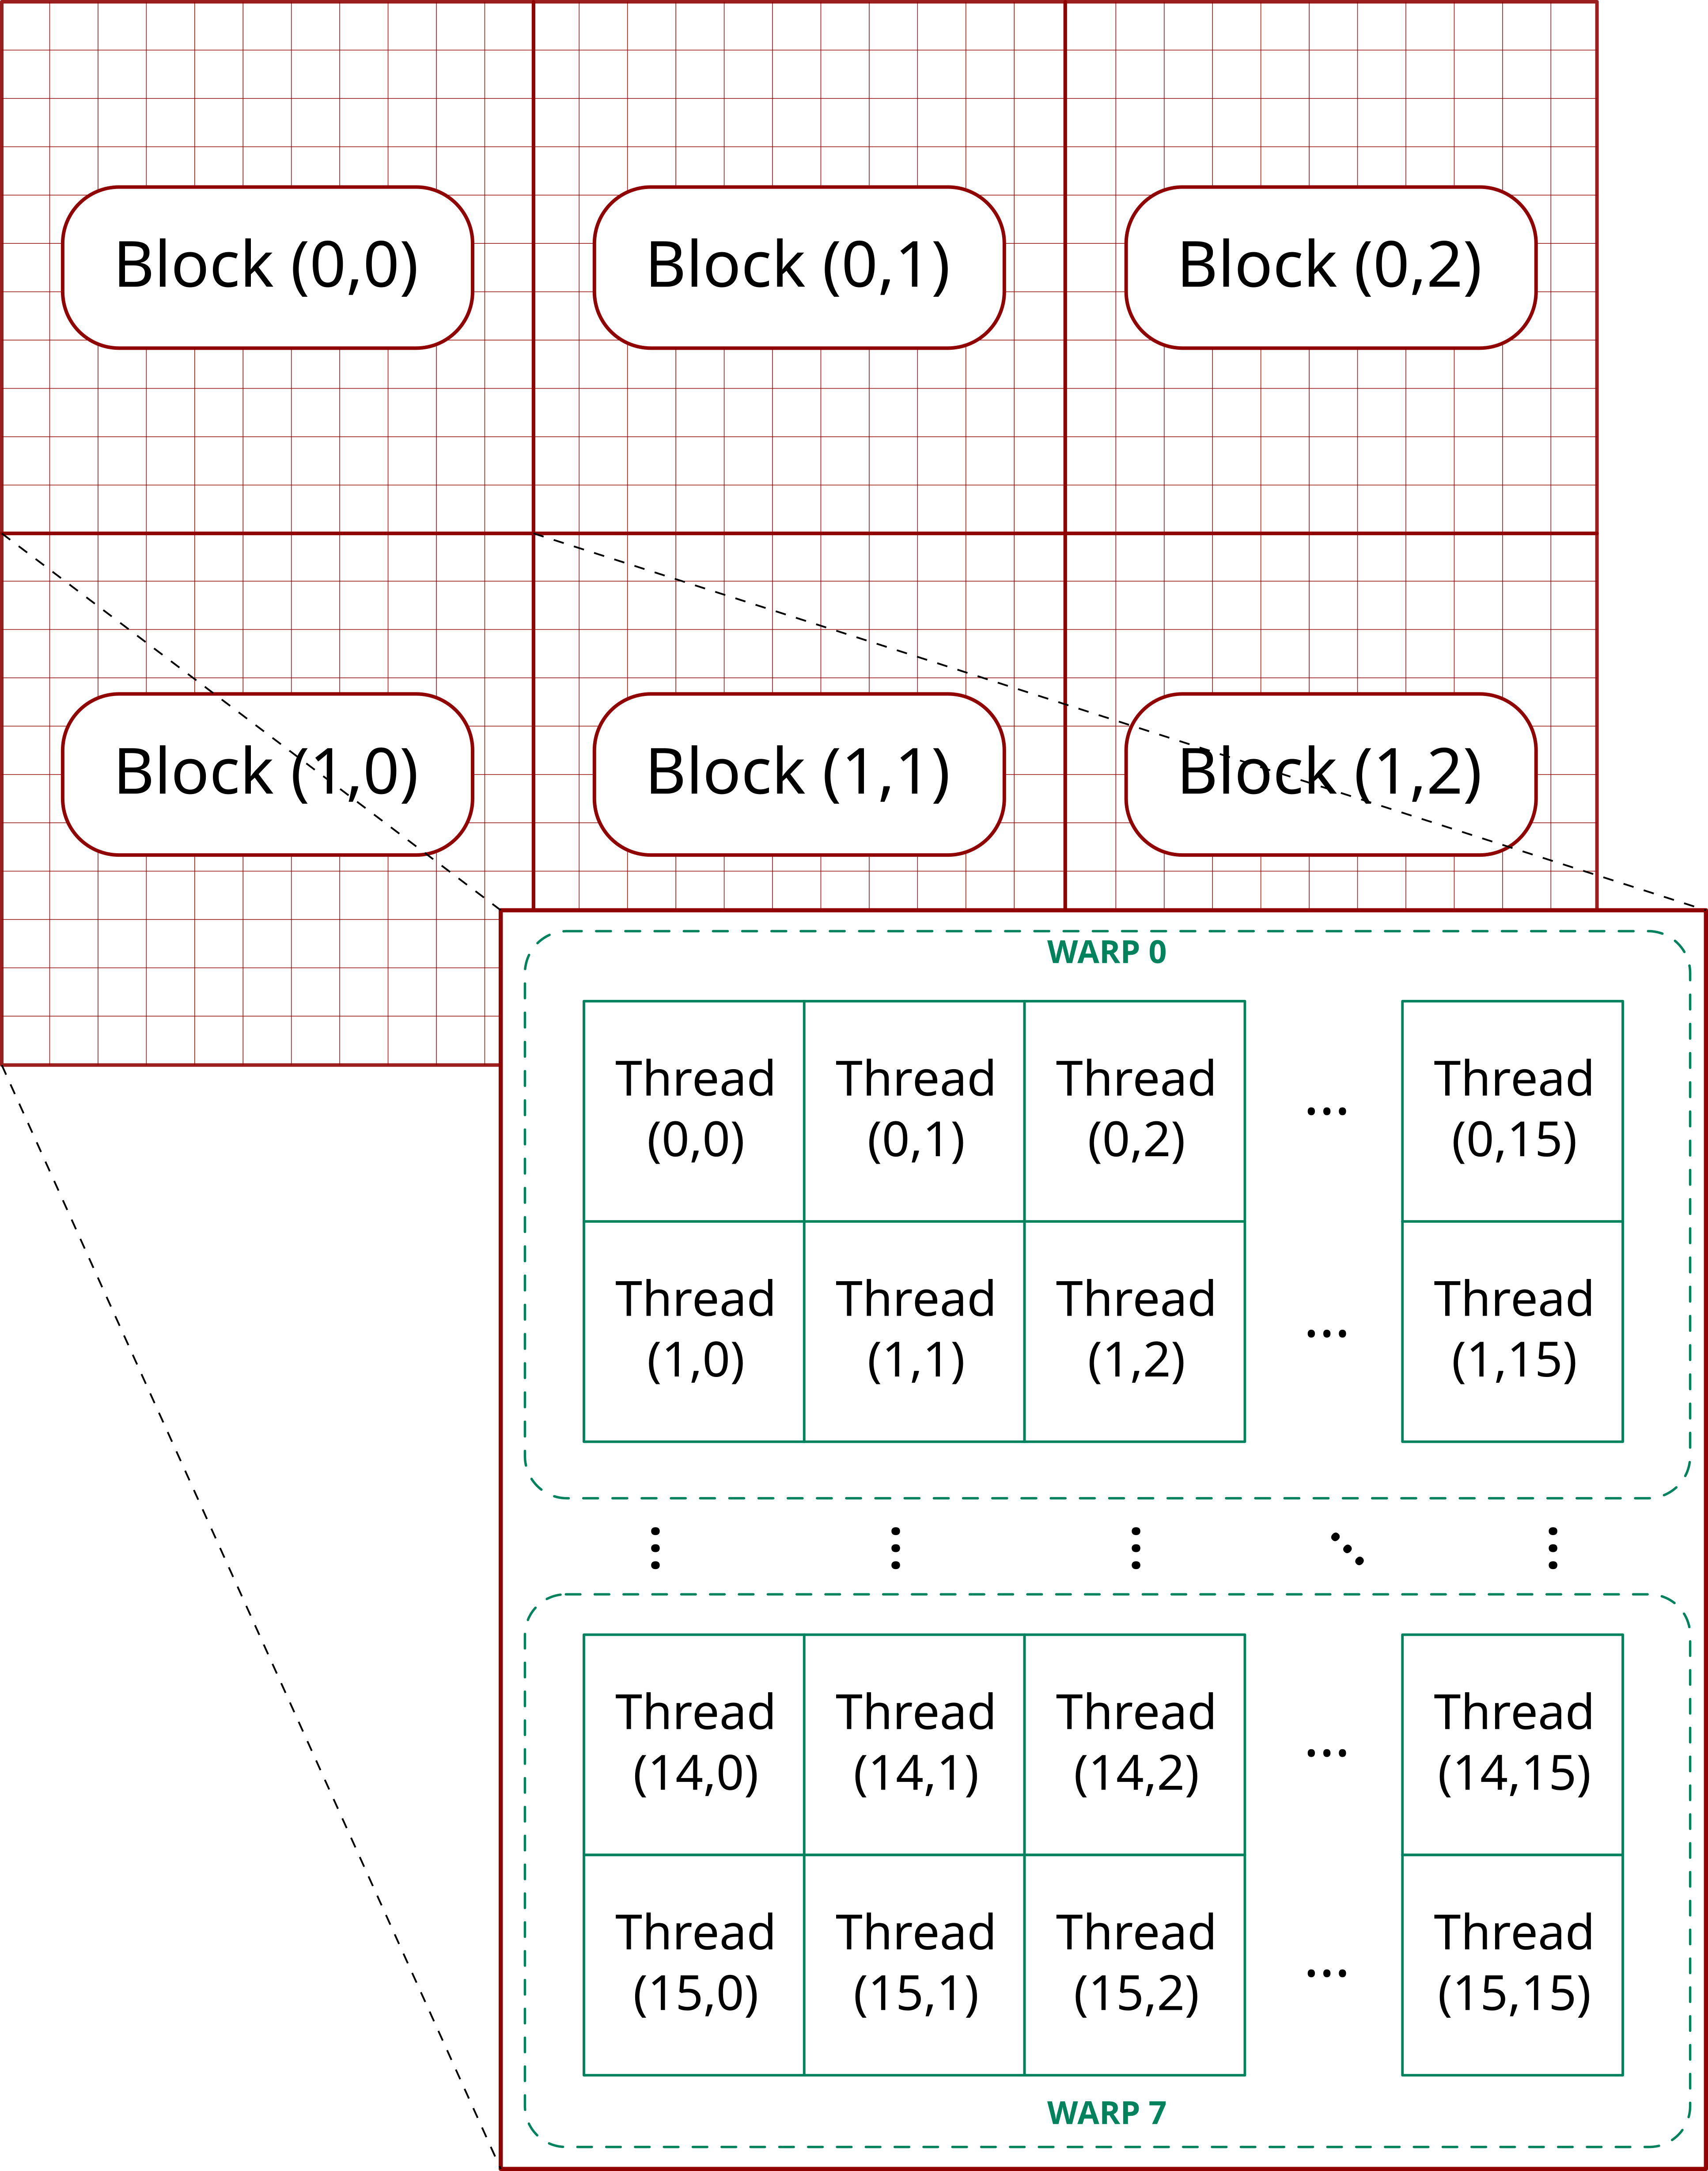
\includegraphics[width=.8\linewidth]{gfx/cudagrid.png}
	\caption[$2\times3$ grid with $16\times16$ blocks]{$2\times3$ grid with $16\times16$ blocks}
	\label{fig:cudagrid}
\end{figure}

An example configuration of the \ac{CUDA} device can be seen on \autoref{fig:cudagrid}, where 6 two dimensional blocks are arranged on the grid in two rows and three columns. Every block has 256 threads, arranged on a 16$\times$16 matrix.

The shape of the \ac{CUDA} grid and blocks are customizable by the user, but the warps are automatically created by \ac{CUDA}, picking up always sets of successive 32 threads, going first through the $X$ axis, then through the $Y$ axis and finally through the $Z$ axis.

This section will study how the grid and blocks are shaped on our software and the implemented parallelized code, as well as some fine-tuning techniques used to speed up the computations.

\subsection{Device Setup}

The configuration of the grid for a ray tracer seems natural. As we are working with images, which are simply two dimensional matrices, the grid will be shaped as a two dimensional matrix, where every thread will compute the geodesic corresponding to a pixel.

The important question now is how to configure the pixels between the blocks; \ie, how to define the number of blocks per column and per row in the grid.

The most simple answer is to define one dimensional blocks of a fixed size that extend along the rows of the image. The very first implementation of the ray tracer used this configuration, but the speed up against the \ac{CPU} implementation was very poor.

The branch divergence was guilty of the poor performance: along a row of the image, the behaviour of the corresponding geodesics is very different, and the so-called \emph{warp divergence} occurs: in a warp ---which in this configuration is defined along the rows of the image---, all threads execute the same instruction at the same time; if the control flow vary between the threads in a warp, some of them will be idle, which causes a great loss of parallel efficiency.

This is avoided by designing a configuration that ensures, or at least that facilitates, that all the threads in a warp execute the same exact code without branch divergence. In our case, this means that the geodesics hitting the pixels in a warp should have followed a nearby path.

However, without knowing a priori the origin of the geodesics, we can only guess which pixels will have similar geodesics. The configuration design follows then this sensible guess: \emph{nearby pixels are hit by geodesics with nearby origins}.

From this assumption, we designed warps as squared as possible, configuring the blocks to have an integer number of warps. This resulted in the following configuration:
\begin{enumerate}
	\item Each block has $8\times8$ threads; \ie, two warps of $8\times4$ threads are located per block. See \autoref{fig:warpconf}.
	\begin{figure}[bth]
		\myfloatalign
		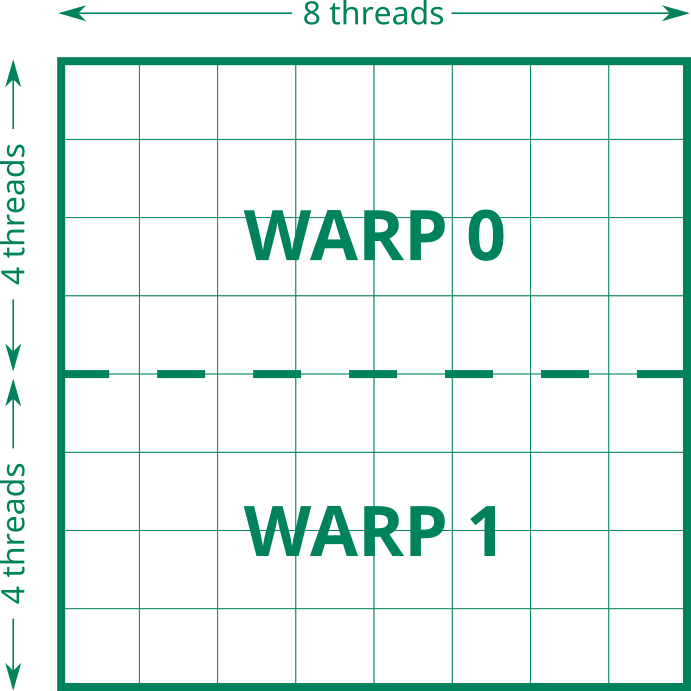
\includegraphics[width=.5\linewidth]{gfx/warpconf.png}
		\caption[Raytracer block configuration]{Raytracer block configuration}
		\label{fig:warpconf}
	\end{figure}
	\item The grid size is dynamically computed using the image size provided by the user. The number of rows and columns of the grid are computed with the following formulas:
	\begin{equation*}
		G_C = \left \lfloor{\frac{I_C - 1}{B_C} + 1}\right \rfloor, \qquad
		G_R = \left \lfloor{\frac{I_R - 1}{B_R} + 1}\right \rfloor,
	\end{equation*}
	where $G_C$ and $G_R$ are the number of blocks per column and per row, $I_C$ and $I_R$ are the columns and rows of pixels of the image and $B_C = B_R = 8$ are the number of columns and rows of a block. These formulas ensure we have enough threads to compute each pixel. The remaining threads, which do not have any geodesic to compute, will be idle during all the program execution.
\end{enumerate}

\subsection{CUDA Kernels}

The main function executed by \ac{CUDA} on the \ac{GPU} is called the \emph{kernel}. Our implementation has three kernels, where every thread is identified with a pixel via its unique identifier in the \ac{CUDA} device. The kernels are:
\begin{enumerate}
	\item \lstinline{setInitialConditions()}: it is the kernel to compute the initial conditions for every pixel, as designed in \autoref{sec:initcond}. From the pixel coordinates, it computes the corresponding pair $(\vartheta_{cs}, \varphi_{cs})$.
	\item  \lstinline{kernel()}: it is the main kernel. It receives the initial conditions for every pixel and the final time until which the \ac{ODE} system will be integrated. It computes the origin of each geodesic, \ie, the pair $(\vartheta', \varphi')$, using the design described at \autoref{sec:numerical}, while continuously checking for collisions with the accretion disk.
	\item \lstinline{generate_image()}: it is an auxiliary kernel to map textures into the images. It receives the origin of the geodesic corresponding to each pixel in the image and maps it to a pixel in the provided texture.
\end{enumerate}

\subsection{Optimizations}

The computational bottleneck of the ray tracer is the \ac{ODE}solver. In particular, the computation of the right hand side of the system ---in terms of the \autoref{sec:numerical}, the function $f(y,t)$---, which involves a lot of operations, some of them really expensive, as the \lstinline{sin()} and \lstinline{cos()} functions.

This chunk of code has been highly optimised, pre-computing all repeated operations and using efficient implementations such as the \lstinline{sincos()} function. The derivatives on equations \ref{eq:eqsmotionp}, \ref{eq:eqsmotionpr} and \ref{eq:eqsmotionpt} have been expressed in their most elementary terms and all common quantities between them have been also pre-computed. To optimise the memory access time, the thread's local memory has been used whenever it was possible.

Furthermore, a specific issue has been taking into account: the \ac{ILP}. It is clear that a single thread cannot keep the \ac{GPU} busy, so the device schedules threads and instructions in such a way that the \ac{GPU} is always busy.

One way of helping the \ac{CUDA} scheduler to maximize the device occupancy is to design the code optimising the \ac{ILP}.

All the ray tracer implementation is coded in such a way that independent instructions are together, whereas dependent ones are as far as possible one of the other. This let the scheduler issue instructions in parallel without having to wait for dependent computations to finish.

In particular, the code of the computation of $f(y,t)$ has been deeply studied in order to maximize the \ac{ILP}.